% !TEX encoding = UTF-8
% !TEX TS-program = pdflatex
% !TEX root = ../thesis.tex

%************************************************
\chapter{The Higgs as a Window to New Physics}\label{chap:three}
%************************************************

As we saw in the previous chapter, the Higgs boson has a very special place in the \acs{SM}, giving rise to the masses of all other elementary particles. But the fascinating properties of the Higgs boson do not end with the \acs{SM}. In fact many of the properties of the Higgs boson puzzle physicists to this day, but they can also serve as guidelines to look for physics beyond the \acs{SM}. The minimal supersymmetric \acs{SM} (\acs{MSSM}) for example was primarily proposed to solve the hierarchy problem, \ie\ the problem of why the Higgs mass is so much smaller than the Planck scale. Furthermore, state-of-the-art measurements hint towards a metastable Higgs potential, meaning that the universe could at some point transition to a new \acs{VEV}. The Higgs is also an excellent candidate as a portal to a hidden dark sector, thus possibly explaining the origin of dark matter \acs{DM}.

Although by no means a complete list of Higgs physics research, we want to highlight these three fields---the Higgs portal to \acs{DM}, the stability of the Higgs potential, and the Hierarchy problem---and briefly review them in the following chapter. It will also underscore the importance of precision calculations in the \acs{SM}

\section{Higgs Portal}
Every particle in the \acs{SM} was uniquely characterized by its mass, spin, the various quantum numbers under the $\SU{3}_C \times \SU{2}_L \times \U{1}$ gauge group. For example, the left-handed up-quark is in a color triplet, has isospin $+1/2$, and weak hypercharge $4/3$, whereas the right-handed electron is charged only under the $\U{1}$ group, with hypercharge $-2$. It is therefore conceivable, maybe even plausible, that particles could be neutral with respect to all \acs{SM} gauge interactions. In fact, the right-handed neutrino we introduced in section~\ref{sec:2:EW_symmetry_breaking} was exactly that. Furthermore, there is strong astrophysical and cosmological evidence for the existence of additional matter that does not, or at least not often, interact with the \acs{SM} (see Ref.~\cite{Cirelli:2024ssz} for an overview). This type of matter has the oblique name: dark matter. The nature of this type of matter is still an open question in physics, and countless models have been proposed, explaining it.

A very often broad up model, are so Higgs-portal models. Here, the \acs{DM} interacts with \acs{SM} primarily via Higgs, thus explaining the name. This way, two \acs{SM}, could annihilate into two \acs{DM} particles for instance (see Fig.~\ref{fig:3:Higgs_portal}).
\begin{figure}[h]
\centering
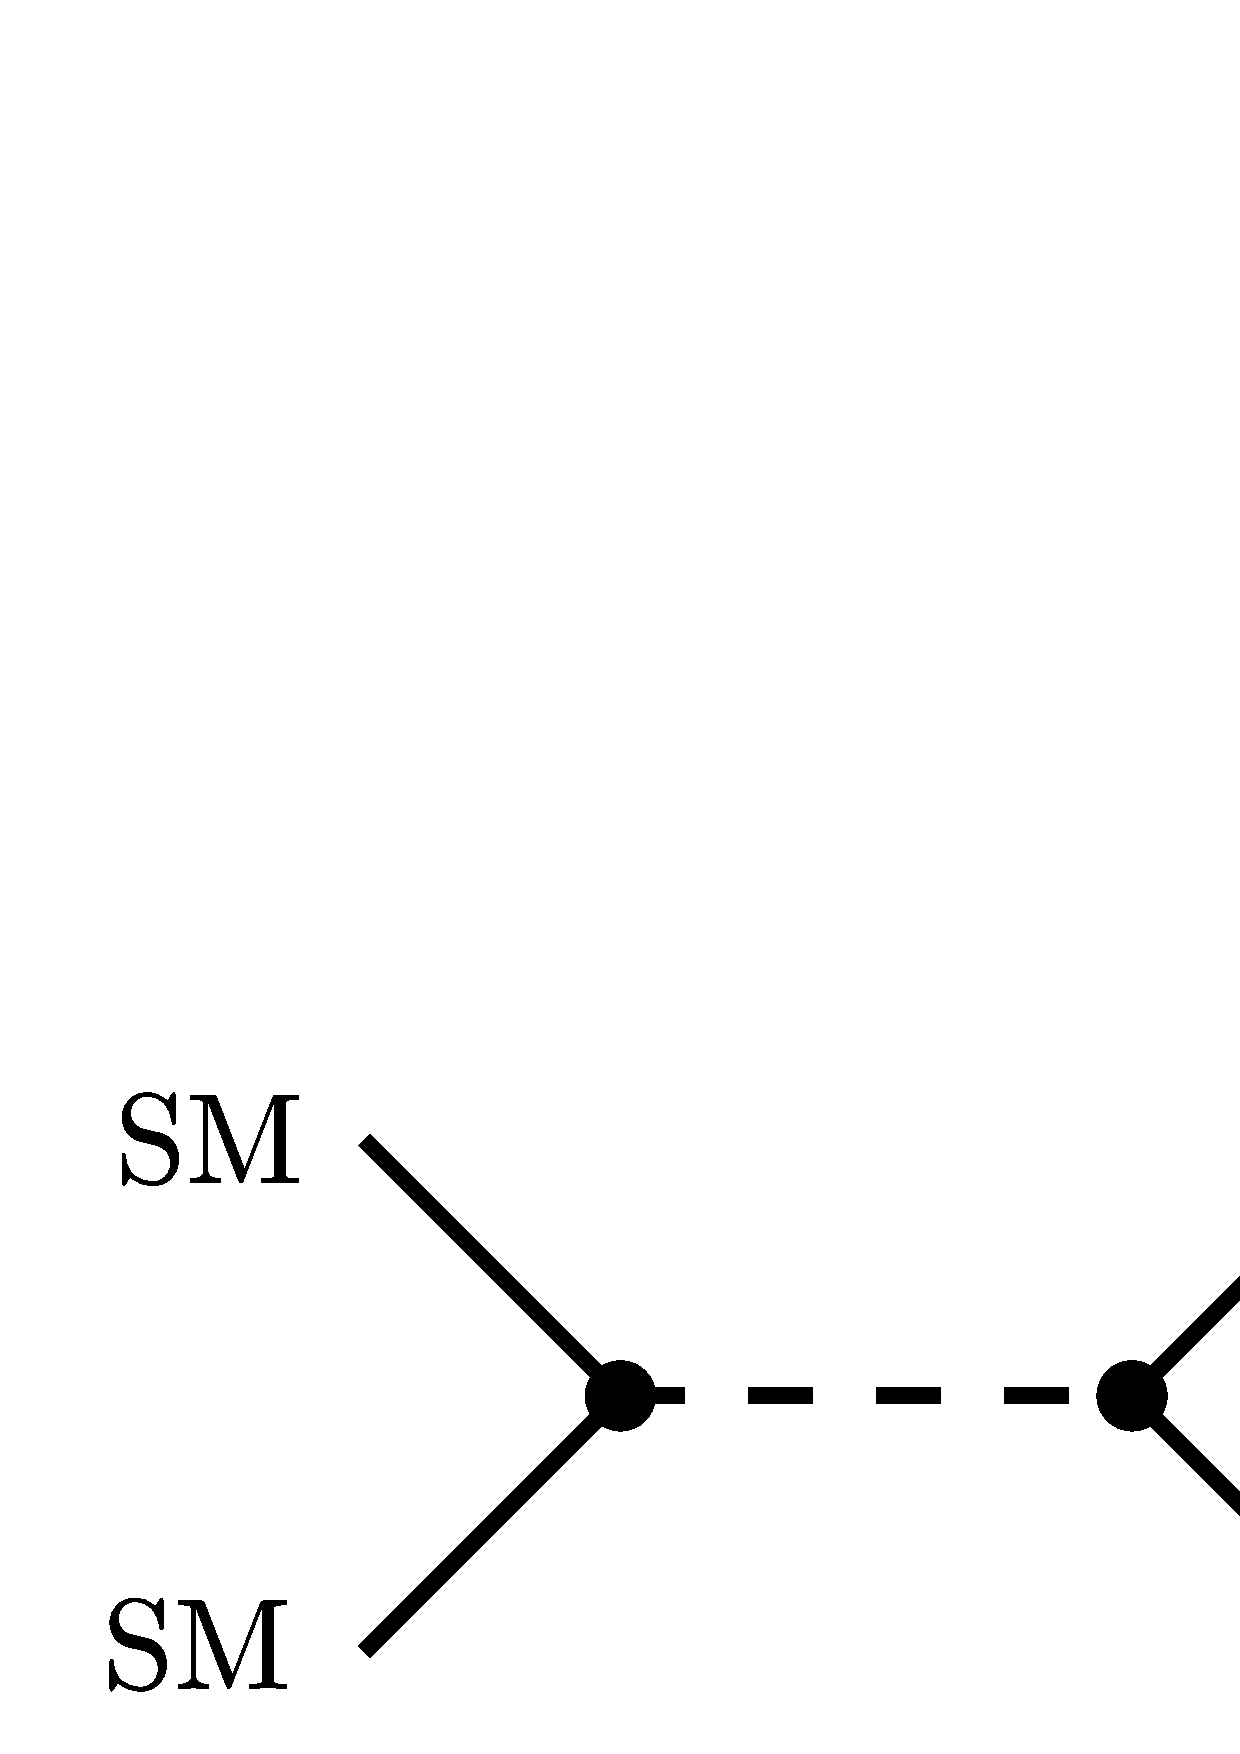
\includegraphics[scale=0.2]{Images/Higgs_portal.pdf}
\caption{Feynman diagram of \acs{SM} particles decaying into \acs{DM} particles via a Higgs portal.}
\label{fig:3:Higgs_portal}
\end{figure}

Since the \acs{DM} is a singlet with respect to the $\SU{2} \times \U{1}$ group, a mass term would not generally break the gauge invariance, \ie\ the mass of the \acs{DM} particles does not have to be, or at least not exclusively, generated through the Higgs mechanism. The Lagrangian of a real scalar, a \textit{Dirac fermion}, and a real vector \acs{DM} field can therefore have the general structure
\begin{equation}
\begin{split}
\mathcal{L}_S &= \frac{1}{2} \left(\partial_\mu S \partial^\mu S - M_S^2 S^2 \right)  - \frac{1}{4} \lambda_S S^4 - \frac{1}{4} \lambda_{HSS} \Phi^\dagger \Phi S^2 , \\
\mathcal{L}_\chi &=  \bar{\chi} \left(i \slashed{\partial} - M_\chi \right) \chi - \frac{1}{2} \frac{\lambda_{H\chi \chi}}{\Lambda} \Phi^\dagger \Phi \bar{\chi} \chi, \\
\mathcal{L}_V &=  - \frac{1}{4} V_{\mu \nu} V^{\mu \nu} + \frac{1}{2} M_V^2 V_\mu V^\mu + \frac{1}{4} \lambda_V \left(V_\mu V^\mu \right)^2 + \frac{1}{4} \lambda_{HVV} \Phi^\dagger \Phi V_\mu V^\mu, \quad V_{\mu \nu} = \partial_\mu V_\nu - \partial_\nu V_\mu.
\end{split}
\label{eq:3:DM_Lagrangians}
\end{equation}
Here, $\lambda_{HSS}, \lambda_{H\chi\chi}$, and $\lambda_{HVV}$ are the dimensionless couplings of the particles to the Higgs, while $\Lambda$ is the new physics scale. The self-interaction terms proportional to $S^4$ and $V^2$ are not important for our purposes. To arrive at Eq.~\eqref{eq:3:DM_Lagrangians}, we postulated, that the Lagrangians respect a $\mathbb{Z}_2$ symmetry, that is the symmetry under which all \acs{SM} particles are symmetric, and all \acs{DM} particles are antisymmetric. This way, it is ensured, that every vertex must have an even number of \acs{DM} particles. Consequently, the lightest new particle will be stable, and hence present an excellent \acs{DM} candidate. The Lagrangian of a \textit{Majorana fermion} would be $1/2 \mathcal{L}_\chi$. Notably, the fermion Lagrangian is not renormalizable, due to the dimensionful coupling introduced by the new physics scale $\Lambda$. Nevertheless, the effective Lagrangian is rather convenient to parametrize the effects of new physics at some higher scale. The masses of the new particles are now generated partly through the Higgs mechanism, and partly through plain mass terms, such that the total masses reads
\begin{equation}
\begin{split}
m_S^2 &= M_S^2 + \frac{1}{4} \lambda_{HSS} v^2, \\
m_\chi &= M_\chi + \frac{1}{4} \frac{\lambda_{H\chi\chi}}{\Lambda} v^2, \\
m_V^2 &= M_V^2 + \frac{1}{4} \lambda_{HVV} v^2.
\end{split}
\end{equation}


\section{Stability of the Higgs Potential}

\section{The Hierarchy Problem}
